
\definecolor{c1a1a1a}{RGB}{26,26,26}
\definecolor{c999999}{RGB}{153,153,153}
\definecolor{cff6600}{RGB}{255,102,0}
\definecolor{cb3b3b3}{RGB}{179,179,179}
\definecolor{navy}{RGB}{0,0,128}


\def \globalscale {1.000000}
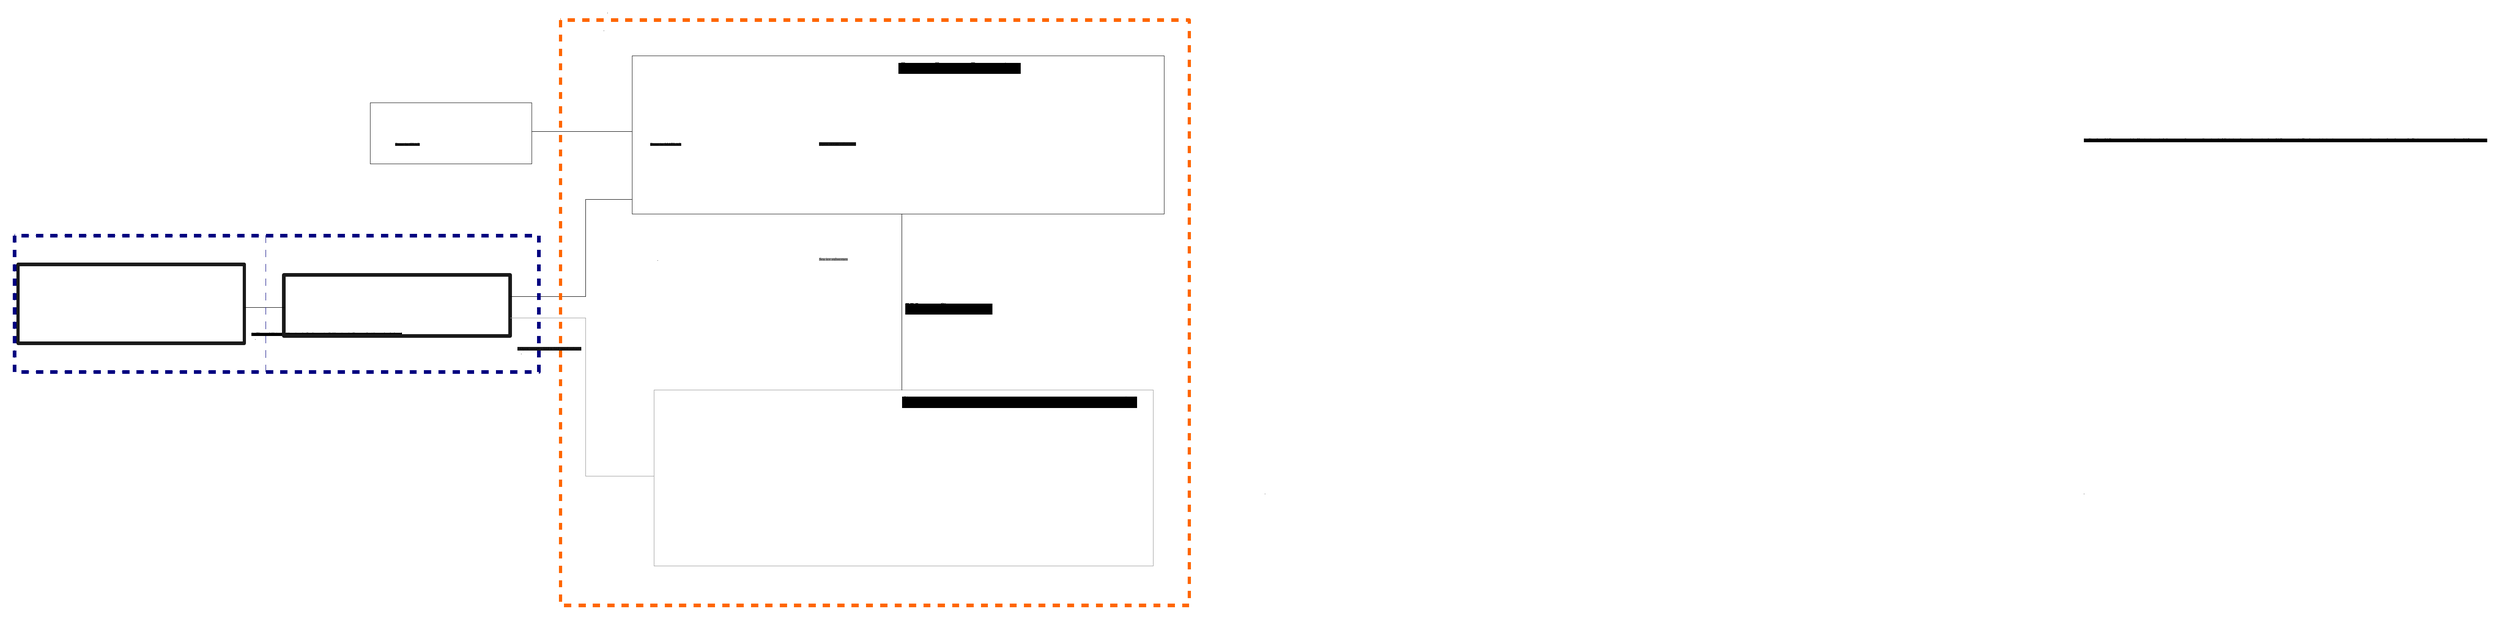
\begin{tikzpicture}[y=1cm, x=1cm, yscale=\globalscale,xscale=\globalscale, inner sep=0pt, outer sep=0pt]
  \path[draw=c1a1a1a,fill=c1a1a1a,fill opacity=0.0,line cap=butt,line
  join=round,line width=0.1cm] (0.2, 22.1) rectangle (6.5, 19.9);
  \node[fill=black,cm={ 0.3,-0.0,-0.0,0.3,(-2.0, 17.6)},anchor=south west]
  (text2) at (8.8, 2.4){};      \node[fill=black,cm={ 0.3,-0.0,-0.0,0.3,(-2.0,
  17.6)},anchor=south west] (text3) at (8.7, 2.5){1. Thermal Noise Calibration
  2. Radiometric Calibration  3. Extract Incidence Angle band};
  \path[draw=c1a1a1a,fill=blue,fill opacity=0.0,draw opacity=1.0,line
  cap=butt,line join=round,line width=0.1cm] (7.6, 21.8) rectangle (13.9, 20.1);
  \node[fill=black,cm={ 0.3,-0.0,-0.0,0.3,(5.4, 17.2)},anchor=south west]
  (text2-9) at (8.8, 2.4){};      \node[fill=c1a1a1a,cm={
  0.3,-0.0,-0.0,0.3,(5.4, 17.2)},anchor=south west] (text3-5) at (8.7, 2.5){-
  Open ocean  - 512 x 512 pixel subsets};      \path[draw=c1a1a1a,fill=blue,fill
  opacity=0.0,draw opacity=1.0,line cap=butt,line join=round,line width=0.0cm]
  (10.0, 26.6) rectangle (14.5, 24.9);      \node[fill=black,cm={
  0.3,-0.0,-0.0,0.3,(7.8, 22.0)},anchor=south west] (text2-9-0) at (8.8, 7.1){};
  \node[fill=c1a1a1a,cm={ 0.3,-0.0,-0.0,0.3,(7.8, 22.1)},anchor=south west]
  (text3-5-9) at (8.7, 6.5){};      \node[fill=c1a1a1a,cm={
  0.3,-0.0,-0.0,0.3,(13.8, 18.9)},anchor=south west] (text3-5-9-5-1) at (8.7,
  6.5){Open ocean subscenes};      \node[fill=c1a1a1a,cm={
  0.3,-0.0,-0.0,0.3,(9.3, 15.7)},anchor=south west] (text3-5-9-5-1-9) at (8.7,
  6.5){};      \node[fill=c1a1a1a,cm={ 0.3,-0.0,-0.0,0.3,(9.1,
  18.9)},anchor=south west] (text3-5-9-5-1-9-0) at (8.7, 6.5){Done in MATLAB};
  \node[fill=c1a1a1a,cm={ 0.3,-0.0,-0.0,0.3,(2.0, 18.9)},anchor=south west]
  (text3-5-9-5-1-9-0-5) at (8.7, 6.5){Done in SNAP};   \node[fill=c999999,cm={
  0.3,-0.0,-0.0,0.3,(13.8, 15.7)},anchor=south west]   (text3-5-9-5-1-2) at
  (8.7, 6.5){Sea ice subscenes};      \path[draw=black,even   odd rule,line
  cap=butt,line join=miter,line width=0.0cm] (6.5, 20.9) -- (7.6,   20.9);
  \path[draw=c1a1a1a,fill=blue,fill opacity=0.0,draw   opacity=1.0,line
  cap=butt,line join=round,line width=0.0cm] (17.3, 27.9)   rectangle (32.1,
  23.5);      \node[fill=black,line width=0.0cm,anchor=south   west] (text6) at
  (24.7, 27.4){Open Ocean Inversion};   \node[fill=black,cm={
  0.3,-0.0,-0.0,0.3,(-0.2, 20.3)},anchor=south west]   (text7) at (57.9, 5.2){1.
  Simulate SAR spectrum ( 2. Use in-situ wind data to   confirm wave direction
  3. Minimise observed vs. simulate SAR spectra  4.   Further minimisation w.r.t
  propogation direction of peak wave  5. Estimate   wave spectrum from SAR
  spectrum};      \path[draw=c999999,fill=blue,fill   opacity=0.0,draw
  opacity=1.0,line cap=butt,line join=round,line width=0.0cm]   (17.9, 18.6)
  rectangle (31.8, 13.7);      \node[fill=black,line   width=0.0cm,anchor=south
  west] (text6-9) at (24.8, 18.1){Sea Ice Inversion   Wave propogation model};
  \node[fill=black,cm={ 0.3,-0.0,-0.0,0.3,(-0.2,   10.5)},anchor=south west]
  (text7-6) at (57.9, 5.2){};   \path[draw=black,even odd rule,line
  cap=butt,line join=miter,line width=0.0cm]   (24.8, 23.5) -- (24.8, 18.6);
  \node[fill=black,line   width=0.0cm,anchor=south west] (text19) at (24.9,
  20.7){Wave Spectrum};   \path[draw=c999999,line cap=butt,line join=miter,line
  width=0.0cm] (13.9,   20.6) -- (14.9, 20.6) -- (16.0, 20.6) -- (16.0, 16.2) --
  (17.9, 16.2);   \path[draw=black,line cap=butt,line join=miter,line
  width=0.0cm] (13.9, 21.2)   -- (16.0, 21.2) -- (16.0, 23.9) -- (17.3, 23.9);
  \path[draw=cff6600,fill=cb3b3b3,fill opacity=0.0,draw opacity=1.0,line
  cap=butt,line join=round,line width=0.1cm,dash pattern=on 0.2cm off 0.2cm]
  (15.3, 28.9) rectangle (32.8, 12.6);      \path[draw=navy,fill=cb3b3b3,fill
  opacity=0.0,draw opacity=1.0,line cap=butt,line join=round,line
  width=0.1cm,dash pattern=on 0.2cm off 0.2cm] (0.1, 22.9) rectangle (14.7,
  19.1);      \path[draw=navy,fill=cb3b3b3,fill opacity=0.0,draw
  opacity=1.0,line cap=butt,line join=round,line width=0.0cm,dash pattern=on
  0.2cm off 0.2cm] (0.1, 22.9) rectangle (7.1, 19.1);   \node[fill=c1a1a1a,cm={
  0.3,-0.0,-0.0,0.3,(26.2, 9.2)},anchor=south west]   (text3-5-9-5-1-4) at (8.7,
  6.5){};      \path[draw=black,even odd rule,line   cap=butt,line
  join=miter,line width=0.0cm] (14.5, 25.8) -- (17.3, 25.8);
\end{tikzpicture}
